\setchapterstyle{kao}
\setchapterpreamble[u]{\margintoc}
\chapter{ Relay 485 Module}
\labch{43R4M}

\section{Function Description}
4 roads IO relay control board with 485 protocal to USB is used for sewage and clean pump open and close control. 


Application: 24v io control.

\begin{figure}[!htb]
	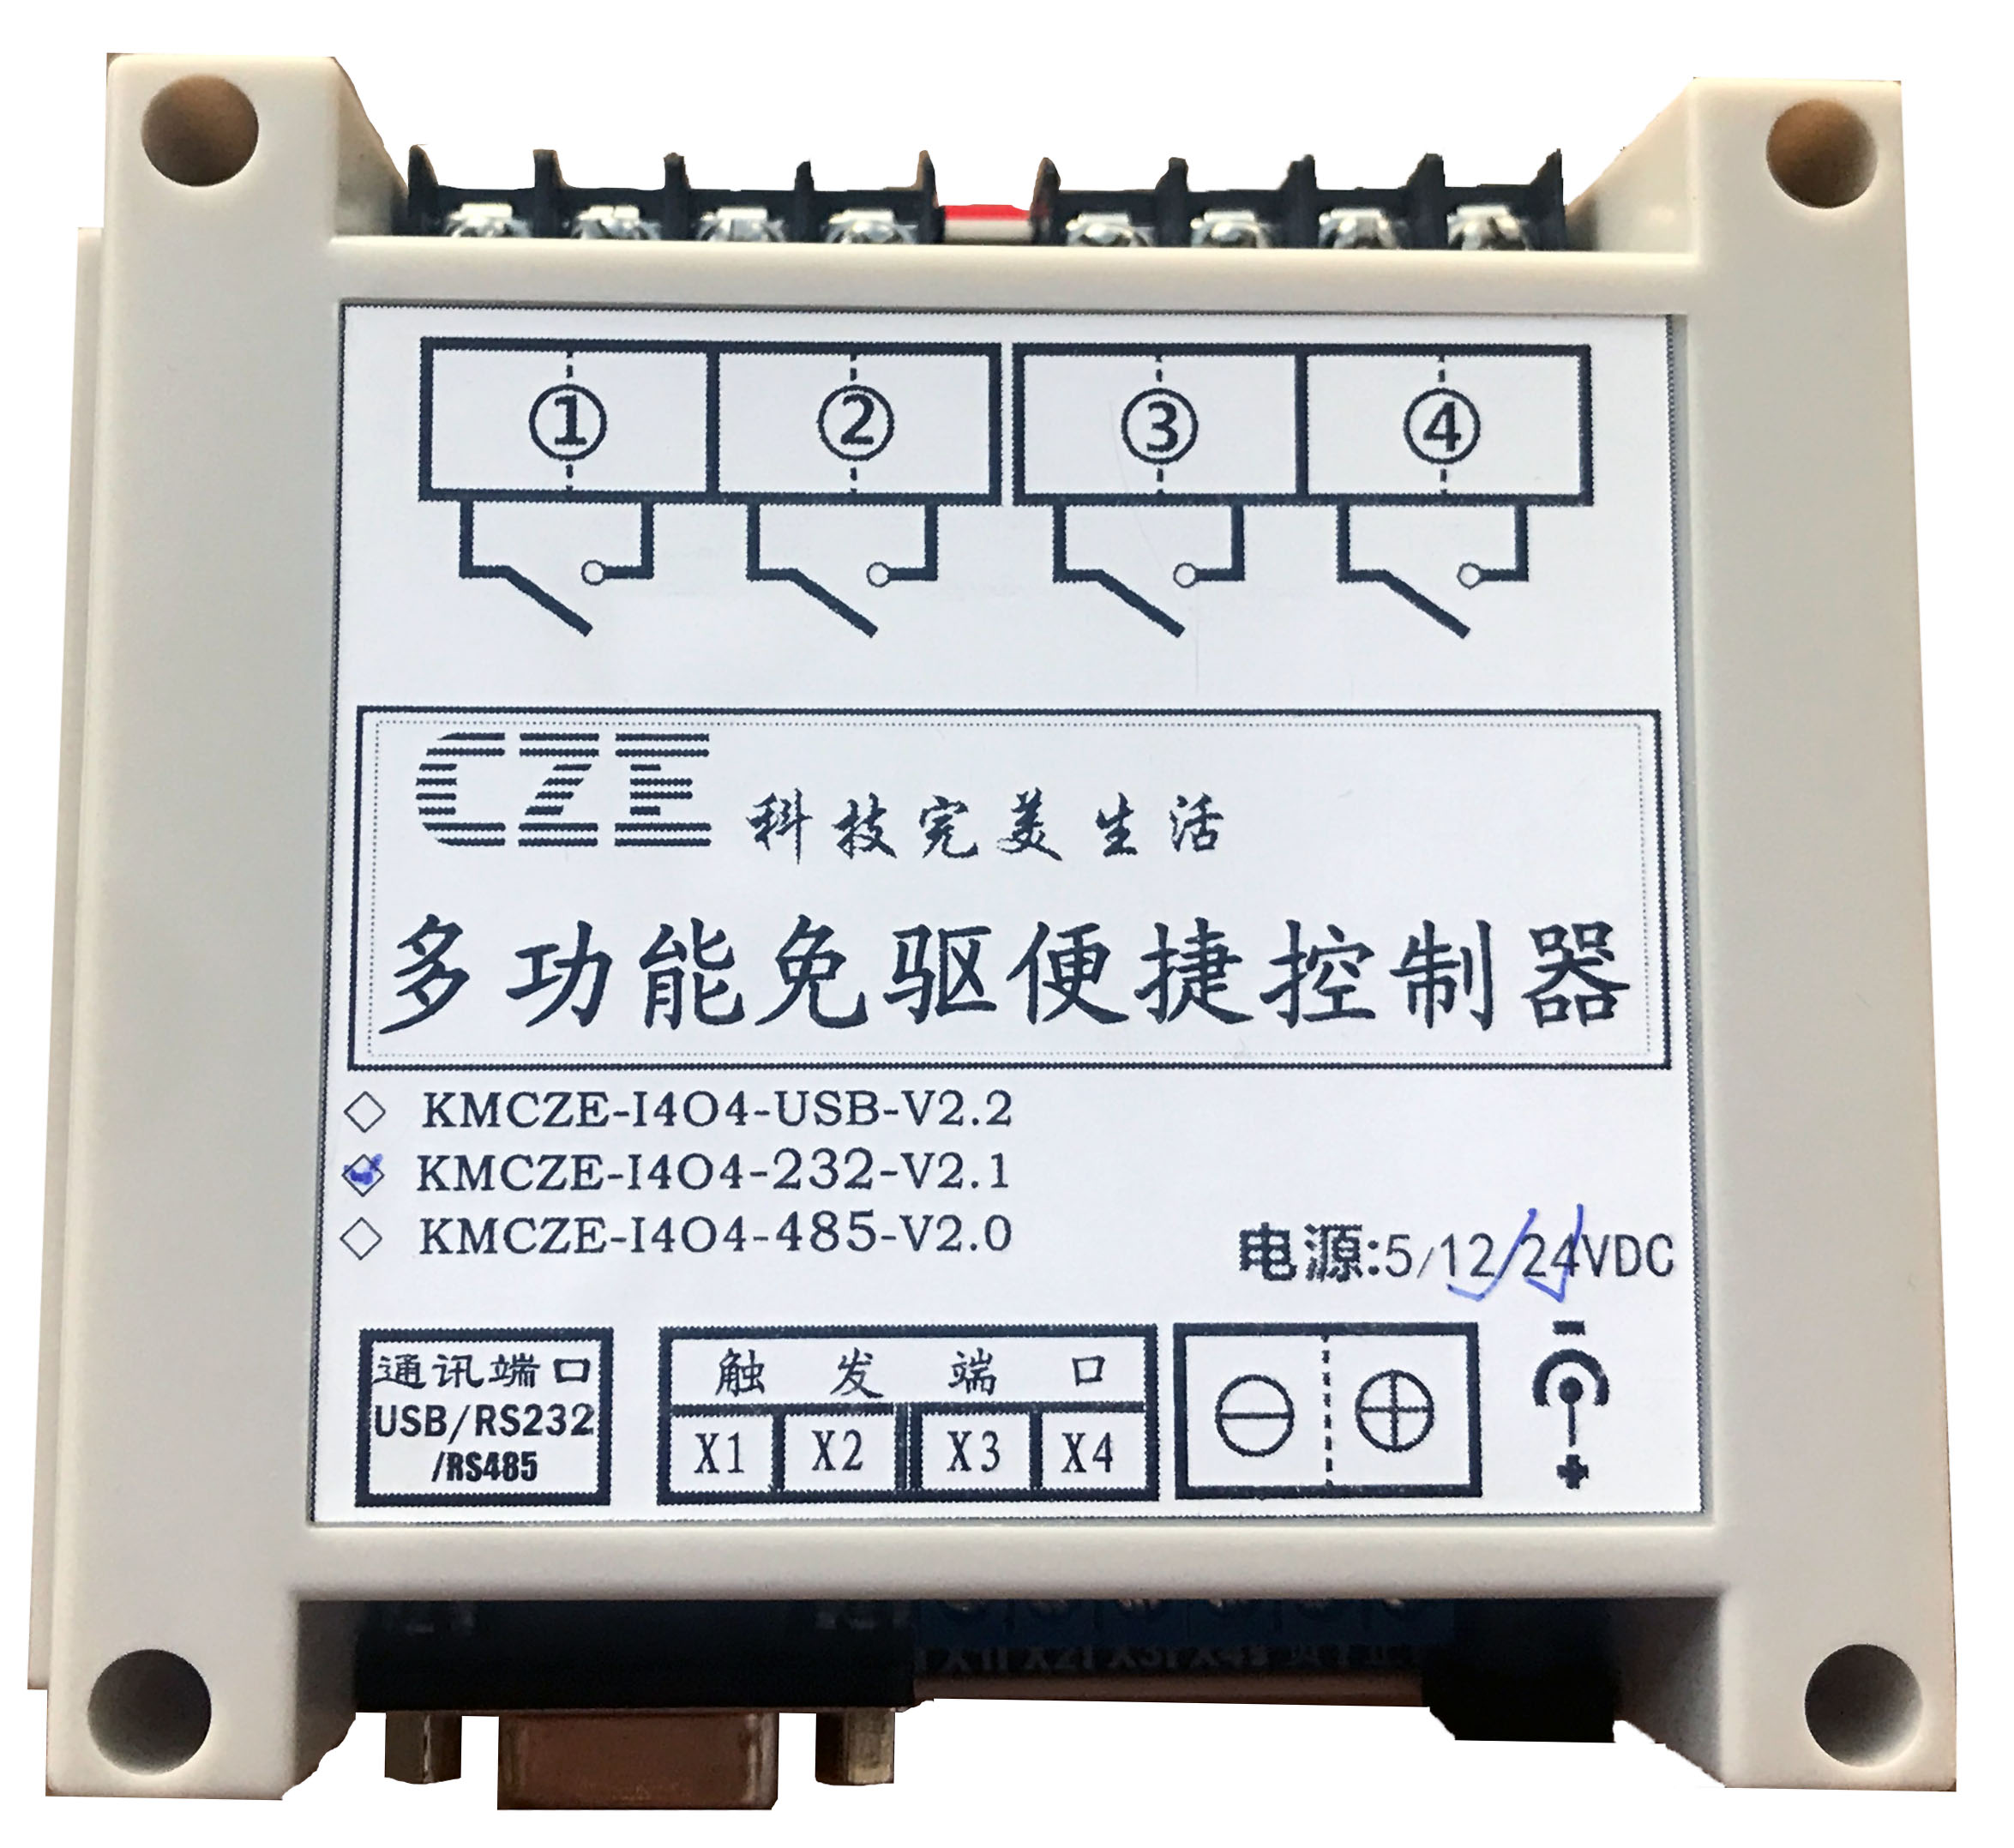
\includegraphics[width=1\textwidth]{43_R.jpg}
	\caption[485 Relay module]{ 
		485 Relay module.		 
		}
	\labfig{fig43_R}
\end{figure}
% \marginnote[-12pt]{
	
% 	}

\section{Purchase Info}
\begin{enumerate}
	\item brand: KMCZE
	\item type: KMCZE-I4O4-U241.0
	\item link: \href{https://item.taobao.com/item.htm?id=559200622128}{taobao link} 
	\item price: 155RMB
	\item data: June. 2020
	\item RP: SGL, clear
\end{enumerate}


\section{Electrical Specification}

\begin{figure}[!htb]
	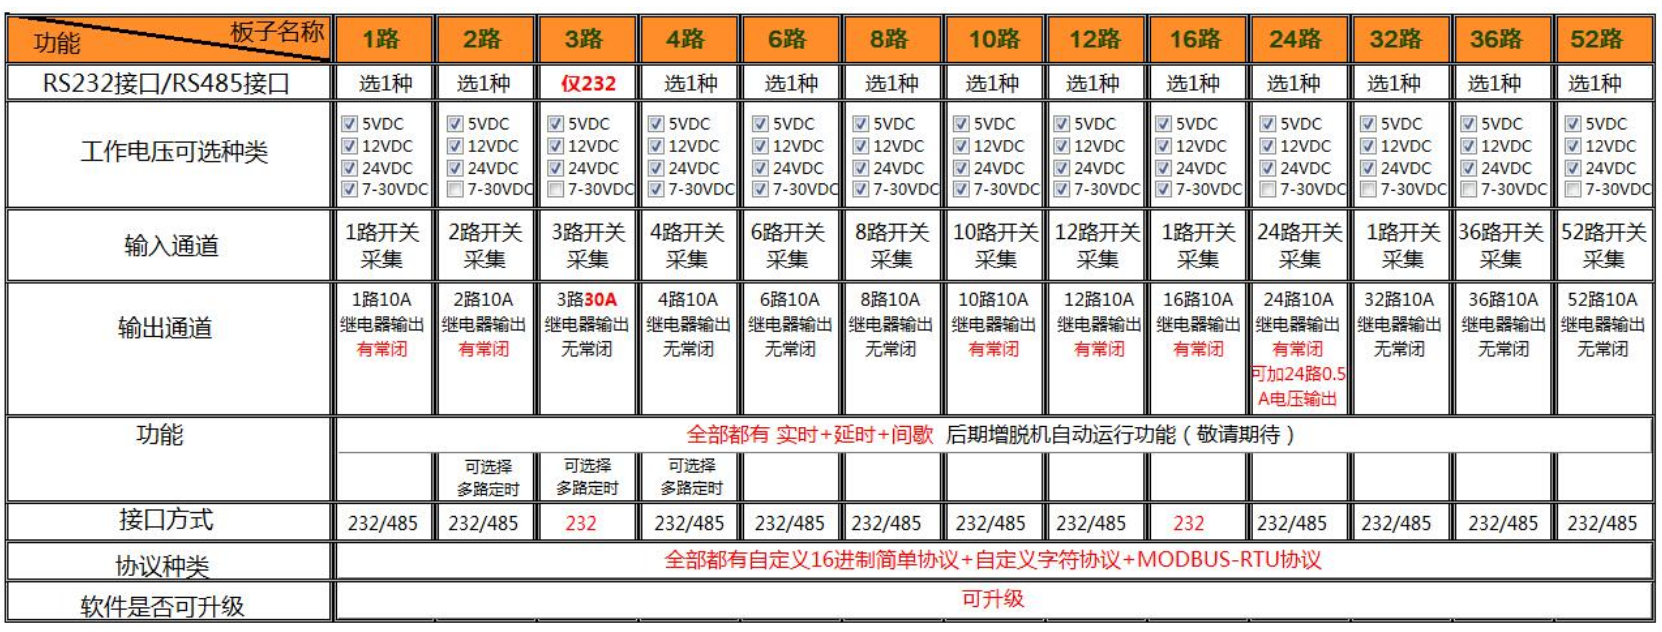
\includegraphics[width=1\textwidth]{433_R_sp.png}
	\caption[ relay electrical specification]{ 
		relay electrical specification, here 4 roads is bought.		 
		}
	\labfig{fig:433_R_sp}
\end{figure}

\begin{enumerate}
	\item power supply: 24v
	\item constant output current: 10A
\end{enumerate}
